\documentclass[letterpaper]{article}
\usepackage[utf8]{inputenc}
\usepackage[parfill]{parskip}    % Activate to begin paragraphs with an empty line rather than an indent
\usepackage{graphicx}
\usepackage{amssymb}
\usepackage{amsmath}
\usepackage{amsthm}

\usepackage{afterpage}

\usepackage{algorithm}
\usepackage{algpseudocode}

\usepackage{verse}

\newtheorem{theorem}{Theorem}[section]
\newtheorem{corollary}{Corollary}[theorem]
\newtheorem{lemma}[theorem]{Lemma}

\theoremstyle{remark}
\newtheorem*{remark}{Remark}

\usepackage{epstopdf}
\usepackage{circuitikz}
\usepackage[separate-uncertainty = true,multi-part-units=single]{siunitx}
\usepackage{booktabs}
\usepackage{enumitem}
\usepackage[toc,page]{appendix}
\usepackage{color}
\usepackage{pgfplots}
\usepackage{pgfplotstable}
\usepackage{caption}
\usepackage{subcaption}
\usepackage{url}
\usepackage{multirow}
\usepackage{makecell}
\usepackage[round]{natbib}   % omit 'round' option if you prefer square brackets
\usepackage{titling}
\usepackage{siunitx}

\usepackage{setspace}
% \doublespacing
\usepackage{float}

\pgfplotsset{compat=1.14}


\usepackage{fancyhdr}

\pgfplotscreateplotcyclelist{grayscale}{
    thick,white!10!black,mark=x,mark options=solid, dashed\\%
    thick,white!20!black,mark=o,mark options=solid\\%
}


\newcommand{\answer}[1]{\framebox{$\displaystyle #1 $}}

 
\pagestyle{fancy}
\fancyhf{}
\rhead{David Shi}
\lhead{CS61C}
\cfoot{\thepage}

\title{Lecture 2 - Notes}
\author{David Shi}
\date{June 2019}
\begin{document}

\maketitle

\section{Overview}
Last time, we covered Number Representation, the idea that bits can be used to represent anything in computers, some signed integer representations as well as overflow. In this lecture, we will begin our dive into the Great Idea of Abstraction for Computer Architecture by introducing the higher-level programming language C and some basic C concepts.

A quick note from the instructors: We will not learn C from lectures alone. For many of us (\textit{including myself}), this is our first time using a language that is not Object Oriented. It is very important to \textbf{Practice} in order to learn the language and get better. My most comfortable languages are Python and Java, and I will quite often compare C to these two languages.

\section{Basic C Concepts}
Let's first cover some of the features of C that distinguishes it from other languages. First, C is a compiled language, similar to Java. The Compiler will take the C code that we write and translate it into Machine code for the computer to run. This is different from Java, since C is making machine code for the physical computer, while java does it for the Java Virtual Machine. This means that C source code cannot be run with similar results across different computers unlike Python and Java.

However, since C code is written specific to its computer architecture, this means that its Run time performance will be the most optimized and will run faster than Java or Python.

The drawback of compilation in C is that executable files must be rebuilt on each individual machine it is being run on. This can be a tedious process when trying to distribute C code.

Variables are also Typed in C. This means that when declaring a variable, the type must be provided, similar to Java. However, variables in C are also "weakly" typed. With our understanding that bits can be used to represent anything, we can typecast our variable from one type to another as we please.

\subsection{Structs}
The main defining feature of C that differentiates itself from Java and Python and most other languages is that it is \textbf{Function Oriented} rather than \textbf{Object Oriented}. This means that C does not have classes like Java and Python do. The closest feature that C has to a class is a \textbf{Struct}. A struct does not have methods like a class does. All that a struct has is a structured group of variables. It is essentially just an abstraction for a group of variables. This is extremely important to understand because for programmers like me who have only learned OOP, we will have to think of C differently.

\section{C Syntax}
We covered some of C specific syntax in Lecture. I will simply refer you to slides 24-34 of the Lecture Slides if interested: 

https://drive.google.com/file/d/1AeNsWBq7KO759bvIbQDDF3LEJPp5Pgf5/view 

There isn't much to elaborate on with the syntax. Some syntax covered include main functions, variable declaration, and true and false values in C.

\section{Pointers}
Our instructor multiple times emphasized that this section of the lecture is \textbf{THE MOST IMPORTANT PART} of the lecture.

\subsection{Address vs. Value}
Let us consider memory as a very large array:

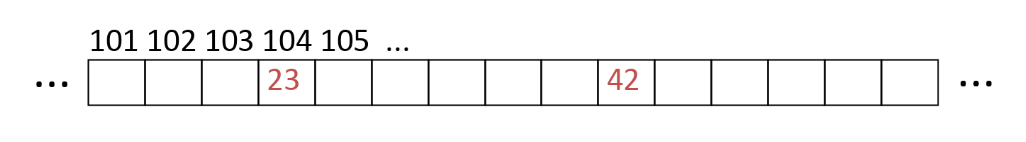
\includegraphics[scale=.5]{Address}

The Address refers to the memory location that a value is stored in, while the value is the value itself. Using our array analogy, the address refers to the index in the array, while the value is the item stored in that index of the array. In the figure above, 104 refers to the Address and 23 is the value stored in that Address. 

It is very important we keep these terms in order.

\subsection{Pointers}
Now that we understand the difference between addresses and values, let us begin to talk about \textbf{Pointers}. A pointer is a variable that contains an address and the variable points to the memory location of a given address. Consider our previous image with a pointer p instantiated:

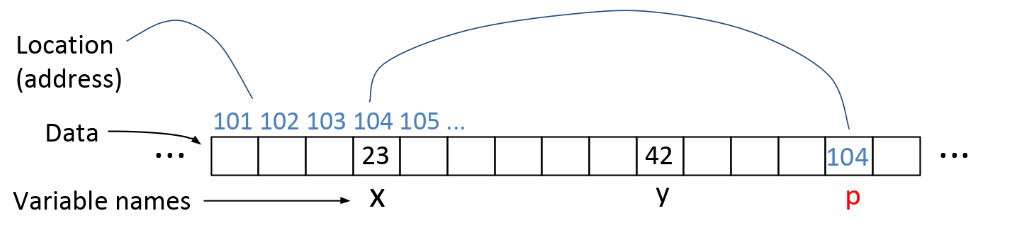
\includegraphics[scale=.5]{pointer}

This image is created with the following lines of code:

    int x;

    int y;

    int *p;

    x = 23;

    y = 42;

    p = &x
    
The important Pointer Syntax shown in this code includes the following: a pointer is declared with 
(type) *p with the * declaring p to be a pointer of type (type). p is assigned to point to the memory location of x with &, as &(var) returns the memory address of (var) if we wanted to find out what value is in the address that pointer p points to, we can \textbf{dereference} p by writing *p. We can potentially change the value inside x by saying *p = (new int), or the dereference value of p will now equal (new int).

\subsection{The importance of Pointers}
The primary reason that pointers are important is because C passes parameters "by value". This means that any changes made to the parameters inside of a function \textbf{WILL NOT} change the original variables. This is why a pointer must be passed in to maintain changes made by a function.

Consider the following code:

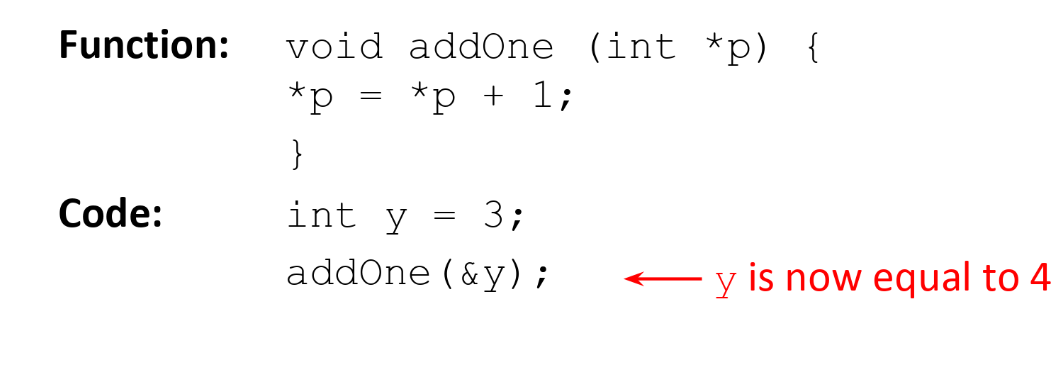
\includegraphics[scale=.5]{byvalue}

If our parameter for the function was just int p rather than int *p, our change made to p within the function will not be saved for the rest of the code. By changing the value stored at the memory location p points to, our change made by the function addOne can be saved for the rest of the code.

Other important reasons for the use of pointers include ease of use and runtime speed when copying large structs or arrays. It is easier to use a pointer to point to a struct or array rather than to spend the time copying the entire struct or array. Pointers also in general allow for cleaner, more compact code.

\subsection{Bugs}
We must be careful when using pointers as they will likely be the number one source of bugs, in terms of memory mismanagement and memory leaks. Also keep in mind that similar to variables, pointers contain garbage when initialized and will contain garbage until the pointer is told what to point to.


\end{document}